\section{Day 16: Compactness, mostly in \texorpdfstring{$\RR^2$}{R2} (Oct. 24, 2024)}
Outfit of the day: stripes of pinstripes
\begin{figure}[h]
    \centering
    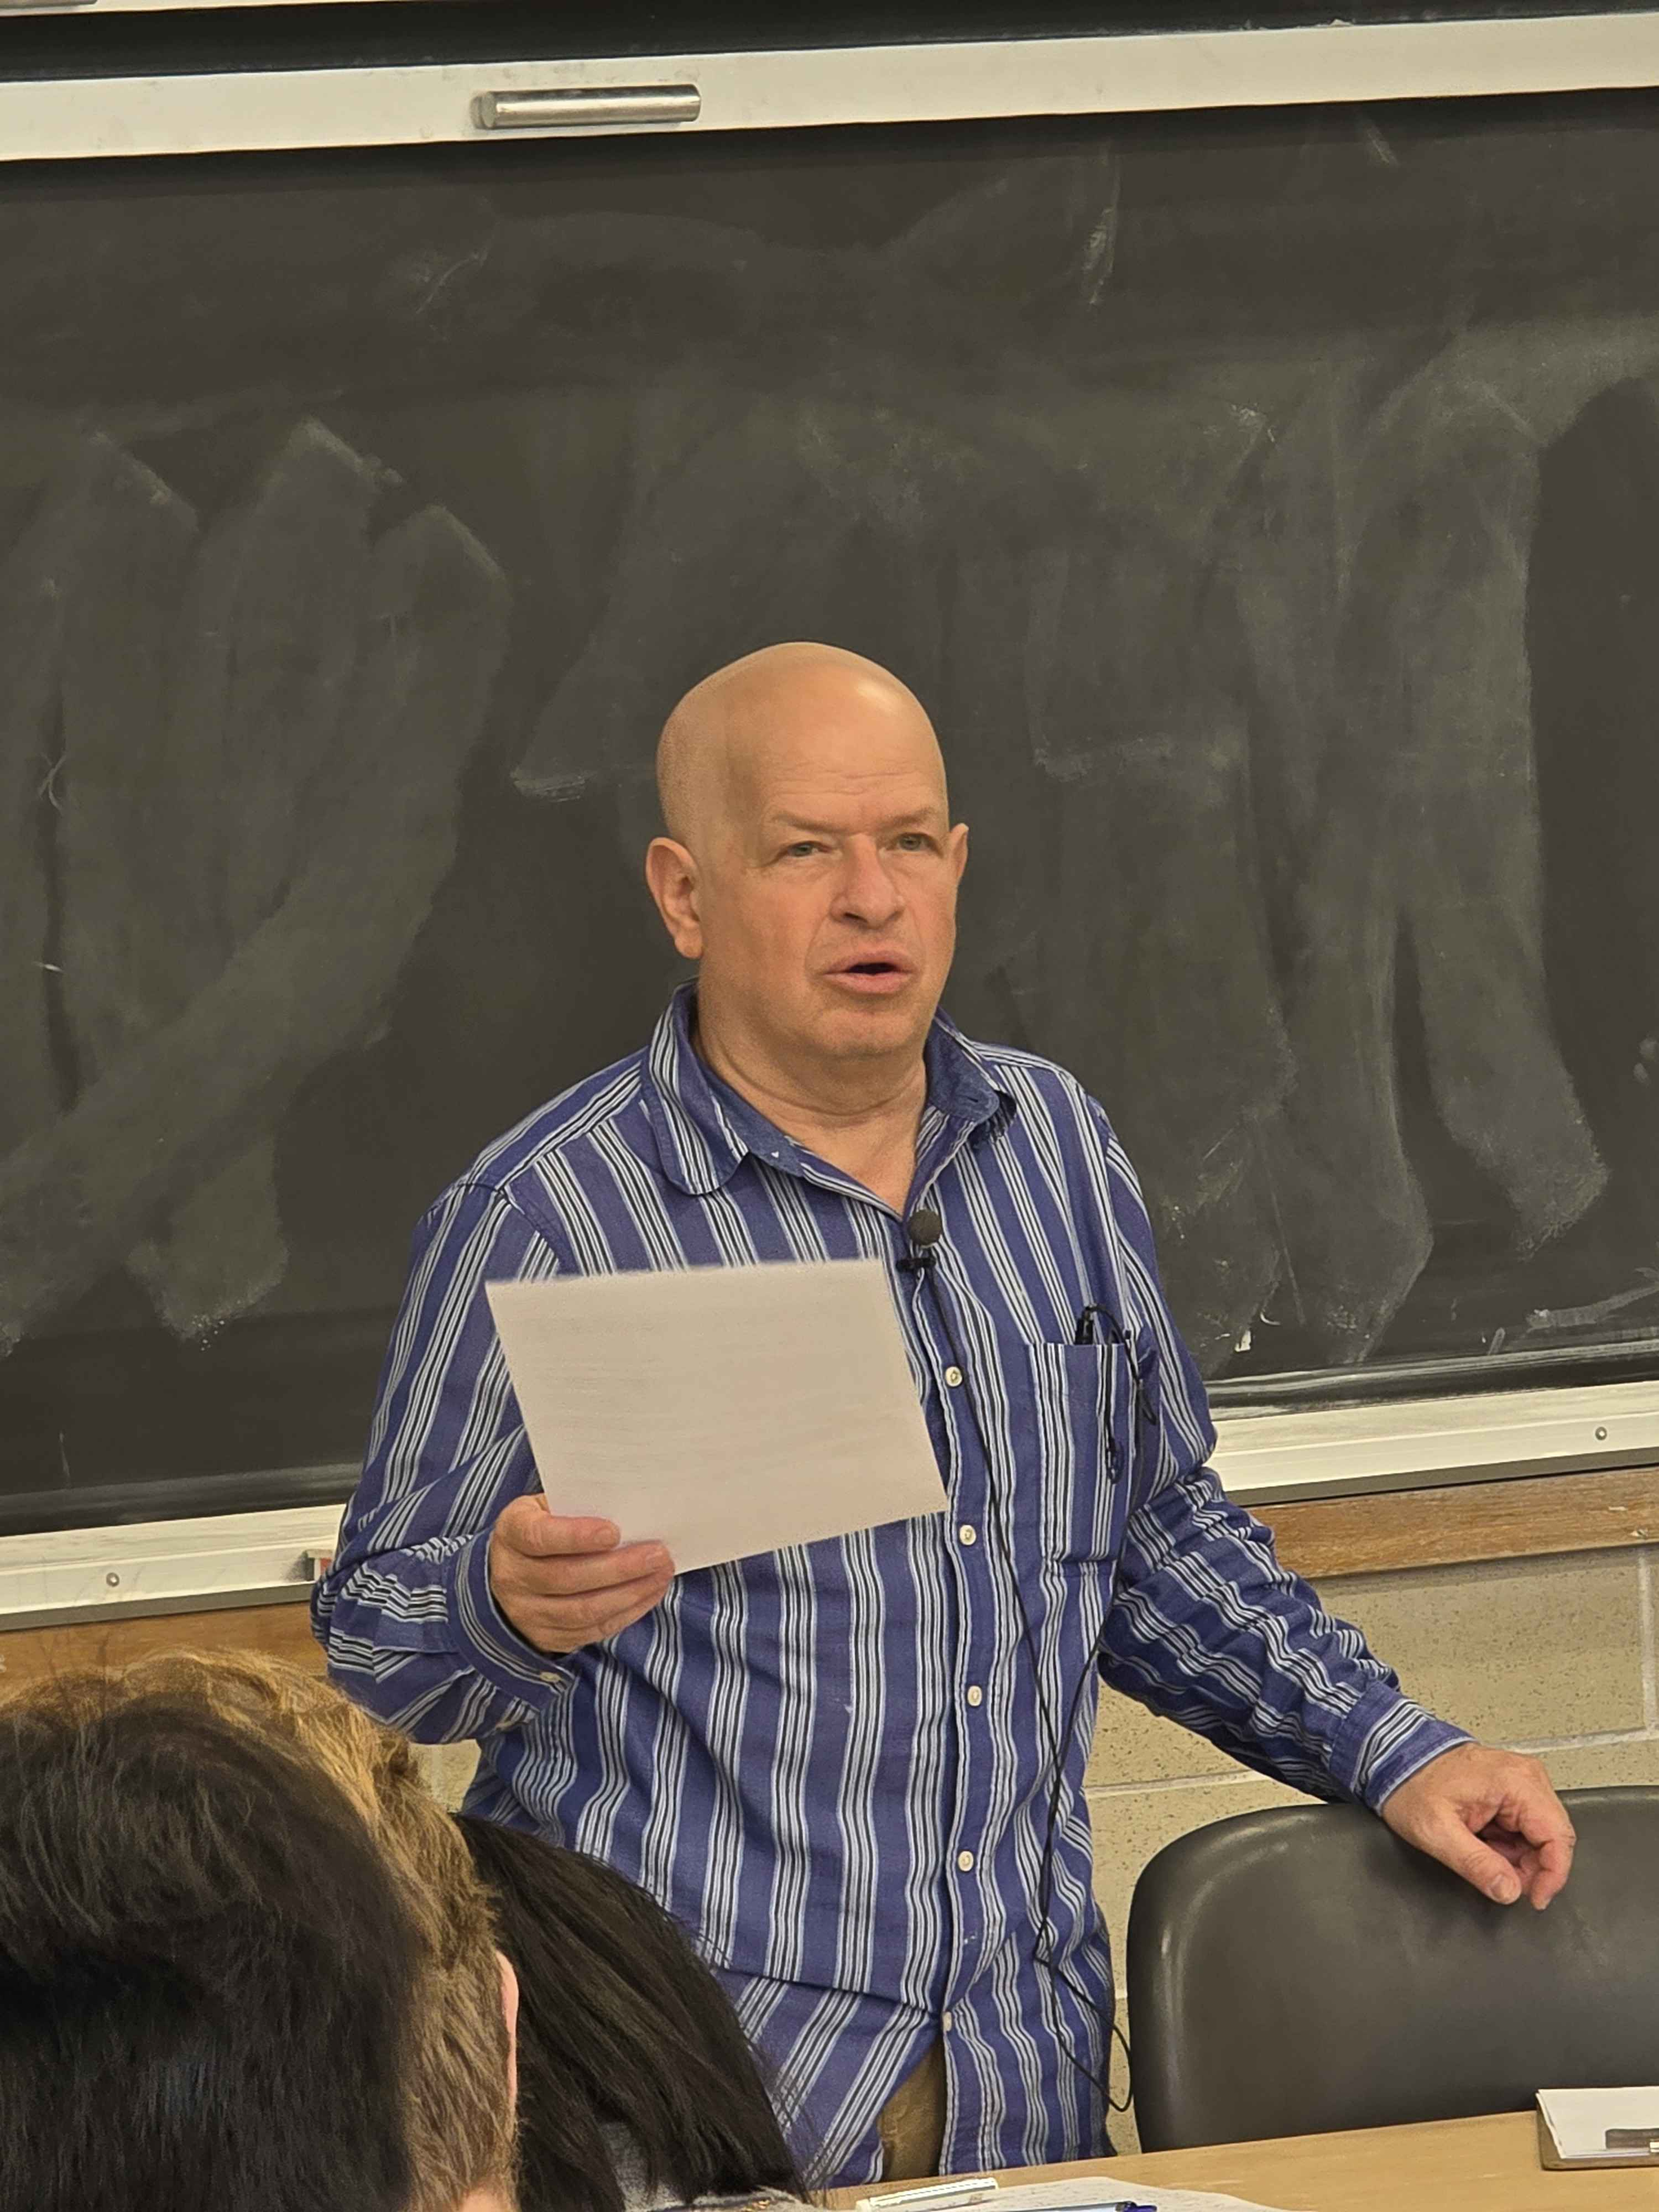
\includegraphics[scale=0.1]{MAT327 Notes/Dror Shirts/dror day 16 shirt.jpg}
\end{figure}

\noindent We define compactness as the property that every open cover of a set $C$ admits a finite subcover.
\begin{simplethm}
    A continuous function on a compact space is bounded.
\end{simplethm}
\begin{simplethm}
    $[0, 1]$ is compact.
\end{simplethm}
\begin{simplethm}
    A closed subset of a compact set is compact.
\end{simplethm}
\noindent The proofs for all three were given in last lecture.
\begin{simplethm}
    A compact subset $C$ of a Hausdorff space $X$ is closed.
\end{simplethm}
\noindent Let $x \in X \setminus C$. By Hausdorffness, for any $y \in C$, there exists open neighborhoods $U_y \ni x, V_y \ni y$ and $U_y \cap V_y = \emptyset$. The colllection $\{V_y \mid y \in C\}$ is an open cover of $C$, so by compactness, it has a finite subcover $\{V_{y_1}, \dots, V_{y_n}\}$. Consider $U = \bigcap_{i=1}^n U_{y_i}$, in which $x \in U$ and $U$ is open. Then
\[ U \cap \bigcup_{i=1}^n V_{y_i} = \bigcup_{i=1}^n (U \cap V_{y_i}) \subset \bigcup_{i=1}^n (U_{y_i} \cap V_{y_i}) \subset \emptyset, \]
so $U$ is disjoint from $C$. \qed
\begin{definition}[Regular / $T_3$]
    A space $X$ is called $T_3$ or \textit{regular} if you can separate points from closed sets: for any $x \in X$ and closed subset $A \subset X$, then there exists open $U, V$ such that $U \ni x$, $A \subset V$, and $U \cap V = \emptyset$.
\end{definition}
\begin{simplethm}
    A compact $T_2$ space is $T_3$.
\end{simplethm}
\noindent Given $x, A$ as per the definition of a regular space, $A$ is a closed subset of a compact space, so it is compact. Now, following the previous proof that a compact subset of a Hausdorff space is closed, let
\[ U = \bigcap U_{y_i}, \hspace{0.2in} V = \bigcup V_{y_i}. \]
This is the desired separation. \qed 
\medskip\newline
\noindent As a corollary, a subset $C$ of $\RR$ is compact if and only if it is closed and bounded (Heine-Borel).
\begin{itemize}
    \item[$(\Leftarrow)$] $C \subset [-M, M]$ for some $M$ by boundedness; since $[-M, M]$ is compact, and $C$ is a closed subset, $C$ is compact.
    \item[$(\Rightarrow)$] By a previous theorem and the fact that $R$ is Hausdorff, $C$ is closed. It is bounded because the union of $(-1, 1), (-2, 2), \dots$ covers $\RR$, and so we may take a finite subcover to contain $C$ to see that it is bounded. The inclusion $i : C \xhookrightarrow{} \RR$ is continuous on a compact set, so it is bounded. \qed
\end{itemize}
\begin{simplethm}
    A continuous image of a compact set is compact, i.e. if $f : A \to Y$ is continuous and $A$ is compact, then $f(A)$ is compact.
\end{simplethm}
\noindent We start with a corollary, aka EVT; if $f : X \to \RR$ is continuous and $X \neq \emptyset$ is compact, then $f$ attains its minimum and maximum, namely, $\exists a, b \in X$ such that for all $x \in X$, $f(a) \leq f(x) \leq f(b)$. We now prove this statement.
\medskip\newline
$f(X)$ is compact, hence it is bounded and closed. Let $m = \inf f(X)$, $M = \sup f(X)$; since $f(X)$ is closed, $m, F \in f(X)$, implying that there exists $a, b$ such that $m = f(a), M = f(b)$. \qed
\medskip\newline
We now prove the original theorem. Let $\SO$ be an open cover of $f(A)$, and consider $\SO' = \{f^{-1}(U) \mid U \in \SO\}$, where we see that $\SO'$ is an open cover of $A$. Since $A$ is compact, there exists a finite subcover of $\SO'$ given by $f^{-1}(U_1), \dots, f^{-1}(U_n)$ for $U_1, \dots, U_n \in \SO$; clearly, $U_1, \dots, U_n$ cover $f(A)$. \qed
\begin{simplethm}
    If $X, Y$ is compact, then $X \times Y$ is compact.
\end{simplethm}
\noindent We consider the reverse direction first;
\begin{itemize}
    \item[$(\Leftarrow)$] This direction is more of a remark if anything; note that the converse of the theorem statement is true only if $X, Y$ are nonempty, since in this case, $\pi_X (X \times Y)$ and $\pi_Y (X \times Y)$ are surjective onto $X, Y$ respectively, and both spaces are continuous images of a compact sets, and so are compact themselves.
    \item[$(\Rightarrow)$] We start by introducing a lemma.
    \begin{simplelemma}[Tube Lemma]
        If $\SO$ is an open cover of $X \times Y$ (with $Y$ compact), and $x \in X$, then there is some open neighborhood $W_x$ of $x$ such that $W_x \times Y$ can be covered with finitely many members of $\SO$.
    \end{simplelemma}
    \noindent We now prove this lemma. Consider $\SO'$ to be the set of $A \times B$, where $A \subset X$, $B \subset Y$, and $A \times B \subset U$ for some open set $U \in \SO$. Clearly, $\SO'$ covers $X \times Y$, so it covers $\{x\} \times Y$. Let us take a finite subcover of $\SO'$, $A_i \times B_i \subset \SO'$ for $i = 1, \dots, n$; without loss of generality, $x \in A_i$ for all $i$ (simple get rid of $A_i \times B_i$ from the finite subcover we're considering if $x \not\in A_i$). Then let $W = \bigcap_{i=1}^n A_i \ni x$, so $W$ is a neighborhood of $x$ as required.
    \medskip\newline
    For each $i$, $A_i \times B_i \in \SO'$, so we may find $U_i \in \SO$ such that $A_i \times B_i \subset U_i$; now,
    \[ \bigcup_{i=1}^n U_i \supset \bigcup_{i=1}^n A_i \times B_i \supset \bigcup_{i=1}^n W \times B_i \supset W \times Y. \qed \]
    We now prove the theorem. By the lemma, let $\SO$ be an open cover of $X \times Y$, and by the lemma, for each $x \in X$, find a neighborhood $W_x$ and $U_{x, 1}, \dots, U_{x, n_x} \in \SO$ where $n_x \in \NN$ such that $W_x \times Y \subset \bigcup_{i=1}^{n_x} U_{x,i}$. Since $\{W_x \mid x \in X\}$ is an open cover of $X$, it has a finite subcover $W_{x_1}, \dots, W_{x_m}$. The set
    \[ \{U_{x_1, 1}, \dots, U_{x_1, n_{x_1}}, U_{x_2, 1}, \dots, U_{x_2, n_{x_2}}, \dots, U_{x_m, 1}, \dots, U_{x_m, n_{x_m}}\} \]
    can be viewed more conveniently by considering each ``cluster'' as $W_{x_1} \times Y \cup \dots W_{x_m} \times Y$ instead, which is equal to $(W_{x_1} \cup \dots \cup W_{x_m}) \times Y = X \times Y$. Thus, $\SO$ has a finite subcover by construction.
\end{itemize}
We now have two corollaries;
\begin{enumerate}[label=(\alph*)]
    \item The product of closed intervals, $\prod_{i=1}^n [a_i, b_i]$, in $\RR^n$ is compact.
    \item $C \subset \RR^n$ is compact if and only if it is closed and bounded.
    \begin{itemize}
        \item[$(\Leftarrow)$] $C$ is closed and bounded, meaning we may take $C \subset \prod_{i=1}^n [-M, M]$ by boundedness; since the product of $[-M, M]$ is compact, $C$ is compact by being a closed subset of a compact set.
        \item[$(\Rightarrow)$] The argument is same as before; we see that $C$ is bounded by considering $C \subset \bigcup_{r > 0} B_r(0)$ and considering a finite subcover of $\SO = \{B_r(0) \mid r > 0\}$; if we consider $n : \RR^n \to \RR$ to be the norm function, i.e. $n(x) = \norm{x}$, we see that it is continuous, hence we have boundedness. \qed
    \end{itemize}
\end{enumerate}
We also talked a bit on Riemann integrals to introduce uniform continuity on arbitrary metric spaces. Define $f : X \to Y$ to be \textit{uniformly continuous} where $X, Y$ are metric spaces, if for all $\eps > 0$, there exists $\delta > 0$ such that for all $x_1, x_2 \in X$ such that $d(x_1, x_2) < \delta$, then $d(f(x_1), f(x_2)) < \eps$.